\chapter{Port-Hamiltonian plate (and shell?) theory}

\epigraph{You get tragedy where the tree, instead of bending, breaks.}{\textit{Culture and Value\\
Ludwig Wittgenstein}}
\minitoc

\lettrine{\color{theme}{P}}lates are plane structural element with a small thickness compared to the planar dimension. Because of the thickness smallness, it is not necessary to model plate structure using three-dimensional models. Therefore, dimensional reduction strategies are employed to model plate structures as two-dimensional problems. These strategies rely on a educated guess of the displacement field. Enough freedom is left so that the assumed field satisfies the equations of elasticity. For beams ans plates the displacement field is expressed in terms of unknown functions $\phi_i^j(x,y,t)$ that solely depends on the midplane coordinates $(x,y)$

\[
u_i(x,y,z,y) = \sum_{j=0}^m (z)^j \phi_i^j(x,y,t).
\]
where $u_{i}$ for $i = \{x, y, z\}$ are the component of the displacement field. The unknown functions are determined so to respect the principle of virtual displacement. In this chapter, the main focus is on the first-order theory. This means that only a linear dependence on $z$ is considered. Two main models arise from such a framework: 
\begin{itemize}
	\item The Kirchhoff-Love model for thin plates;
	\item The Mindlin-Reissner model for thick plates;
\end{itemize}
The interested reader may consult \cite{reddy2006theory} for a detailed monograph on the topic.

\section{First order plate theory}
In this section  the common features of first order plate models are recalled. As previously state first order theories assume a linear dependence on the vertical coordinate
\[
u_i(x,y,z,t) = \phi_i^0(x,y,t) + z \phi_i^1(x,y,t).
\]
This hypothesis implies that the fibers, segments perpendicular to the mid-plane before deformation, remain straight after deformation. Additionally, for plate with moderate thickness the fibers are considered inextensible, meaning that $\phi_z^1 = 0$. These assumption lead to the following displacement field

\begin{equation}\label{eq:disp1or}
\begin{aligned}
u_x(x,y,z,t) &= u_x^0(x,y,t) -z \theta_x(x,y,t), \\
u_y(x,y,z,t) &= u_y^0(x,y,t) -z \theta_y(x,y,t), \\
u_z(x,y,z,t) &= u_z^0(x,y,t), 
\end{aligned}
\end{equation}
where $u_i(x,y,t) = \phi_i^0(x,y,t), \, \theta_i(x,y,t) = -\phi_i^1(x,y,t)$. Assuming a linear elastic behavior, the 3D strain tensor for such a displacement field takes the form
\begin{align*}
\varepsilon_{\alpha \beta} &= \frac{1}{2} \left(\partial_\beta u_\alpha + \partial_\alpha u_\beta \right) - z \frac{1}{2} \left(\partial_\beta \theta_\alpha + \partial_\alpha \theta_\beta \right) = {\varepsilon}^0_{\alpha \beta} - z \kappa_{\alpha \beta}, \\
\varepsilon_{\alpha z} &= \frac{1}{2} \left(\partial_a u_z - \theta_\alpha \right) = \frac{1}{2} \gamma_\alpha,
\end{align*}
where $\alpha=\{x,y\}, \; \beta=\{x,y\}$. The tensors $\bm{\varepsilon}^0,\, \bm{\kappa},\, \bm{\gamma}$ are called membrane, bending (or curvature) and shear strain tensor
\begin{align}
\bm{\varepsilon}^0 &= \Grad \bm{u}^0, \where \bm{u}^0 = (u_x, u_y)^\top,  \\
\bm{\kappa} &= \Grad \bm{\theta}, \where \bm{\theta} = (\theta_x, \theta_y)^\top, \label{eq:kappa}  \\
\bm{\gamma} &= \grad u_z - \bm{\theta}. \label{eq:gamma}
\end{align}

For an isotropic linear elastic material the Hooke's law for 3D continua reads
\[
\bm{\Sigma} = \frac{E}{1+\nu} \left[\bm{\varepsilon} + \frac{\nu}{1-2\nu} \Tr(\bm{\varepsilon})\bm{I}_{3\times 3} \right].
\]
where $E,\, \nu$ are the Young modulus and Poisson ratio. The hypothesis of inextensible fibers leads to $\varepsilon_{zz}=0$. However, imposing a plane strain condition provides a model that is too stiff. Rather than a plain strain assumption, a plain stress hypothesis is used to derive the constitutive law for plates. Setting $\Sigma_{zz}=0$, then one gets
\[
\varepsilon_{zz} = - \frac{\nu}{1 - \nu} (\varepsilon_{xx} + \varepsilon_{yy}).
\]
Consequently, one computes
\[\Tr(\bm{\varepsilon}) = \frac{1 - 2\nu}{1 - \nu} (\varepsilon_{xx} + \varepsilon_{yy}).
\]
The constitutive law for the in-plane stress takes the form
\[
\bm{\Sigma}_{2D} = \bm{\mathcal{D}}_{2D} \, \bm{\varepsilon}_{2D},
\]
where $\bm{\Sigma}_{2D} = \Sigma_{\alpha\beta}, \; \bm{\varepsilon}_{2D} = \varepsilon_{\alpha\beta}$ and 
\[
\bm{\mathcal{D}}_{2D} = \frac{E}{1-\nu^2}\left[ (1-\nu) (\cdot) + {\nu} \Tr(\cdot) \bm{I}_{2\times 2} \right].
\]
Concerning the shear deformation, the constitutive law reduces to 
\begin{equation}
\bm{\sigma}_s = G \bm{\gamma},
\end{equation}
where $\bm{\sigma}_\alpha := \bm{\Sigma}_{\alpha, 3}$ and $G = \frac{E}{2(1 + \nu)}$ is the shear modulus. In the following sections the most common plate model will be presented and discussed.

\subsection{Mindlin-Reissner model}
The Mindlin-Reissner model was formulated by Mindlin in the fifties \cite{mindlin1951}. It represent a first-order shear deformation theory for describing the bending of plate. The in-plane displacement of the mid-plane are assumed to be zero $\bm{u}^0(x,y)=\bm{0}$. Hence, the displacement field assumes the form
\begin{equation}
\begin{aligned}
u_x(x,y,z) &= -z \partial_x \theta_x, \\
u_y(x,y,z) &= -z \partial_y \theta_y, \\
u_z(x,y,z) &= u_z^0(x,y).
\end{aligned}
\end{equation}
In pure bending, the strain tensor is given by
\[
\bm{\varepsilon}_b := \bm\varepsilon_{2D}(\bm{u}^0=\bm{0}) = -z \bm{\kappa},
\]
with $\bm\kappa$ given by \eqref{eq:kappa}. Consequently, the stress tensor reads
\[
\bm{\Sigma}_b := \bm{\Sigma}_{2D}(\bm{u}^0=\bm{0}) = -z \bm{\mathcal{D}}_{2D} \bm{\kappa}.
\]
To effectively reduce the problem from three- to two-dimensional, the stresses have to be integrated along the fibers. Consider an undeformed middle plane of the plate is denoted by $\Omega$. The total domain of the plate is the product $\Omega \times (-h/2, h/2)$, where $h$ is the constant thickness. Since the stress varies linearly, one has to multiply the stress by $z$ to get a non null contribution. Such a quantity is called bending momenta tensor and is given by 
\begin{equation}\label{eq:momenta}
\bm{M} :=-\int_{-h/2}^{h/2} z \bm{\Sigma}_{b} \d{z} = \bm{\mathcal{D}}_{b} \, \bm{\kappa}, 
\end{equation}
where 
\begin{equation}\label{eq:Db}
\bm{\mathcal{D}}_{b} = D_b \left[ (1-\nu) (\cdot) + \nu \Tr(\cdot) \bm{I}_{2\times 2} \right], \where D_b = \frac{E h^3}{12(1-\nu^2)}.
\end{equation}


Furthermore, the shear stress has to be integrated along the fibers. However, given the excessive rigidity of the shear contribution, a correction factor $k=5/6$ \cite[Chapter 10]{reddy2006theory} is introduced 
\begin{equation}\label{eq:shearstress}
\bm{q} = \int_{-h/2}^{h/2} k \bm{\sigma_s} = kGh \bm{\gamma},
\end{equation}


where $\bm{\gamma}$ is defined in Eq. \eqref{eq:gamma}. The equations of motion can be obtained using the Hamilton principle \cite[Chapter 10]{reddy2006theory}. It consists in minimizing the total Lagrangian, given by $L = E_{\text{def}} - E_{\text{kin}} + W$, where $E_{\text{def}}, \, E_{\text{kin}}, \,W$ are the deformation energy, the kinetic energy and the work of external forces respectively
\begin{align}
E_{\text{def}} &= \frac{1}{2} \int_{\Omega} \int_{-h/2}^{h/2} \bm{\Sigma} \cddot \bm{\varepsilon} \d{\Omega} \d{z} = \frac{1}{2} \int_{\Omega} \left\{\bm{M} \cddot \bm{\kappa} + \bm{q} \cdot \bm{\gamma} \right\} \d{\Omega}, \label{eq:defenMin}\\
E_{\text{kin}} &= \frac{1}{2}  \int_{\Omega} \int_{-h/2}^{h/2} \rho \,  \norm{\partial_t \bm{u}}^2 \d{\Omega} \d{z} = \frac{1}{2} \int_{\Omega} \left\{\frac{\rho h^3}{12} \norm{\partial_t \bm{\theta}}^2 + \rho h (\partial_t u_z)^2  \right\} \d{\Omega}, \label{eq:kinenMin}\\
W &= \frac{1}{2}  \int_{\Omega} f u_z \d{\Omega},
\end{align}
where $\rho$ is the mass density and $f$ a distributed surface force. The Hamilton principle states that
\[
\int_{0}^{T} \delta L \d{t} = \int_{0}^{T} \left\{ \delta E_{\text{def}} + \delta W - \delta E_{\text{kin}} \right\} \d{t} = 0.
\]
The final result is the following system of PDEs (for the detailed computations the reader may consult \cite[Chapter 10]{reddy2006theory})
\begin{equation}\label{eq:classMin}
\begin{aligned}
\rho \diffp[2]{u_z}{t} &= \div \bm{q} +  f, \qquad (x,y) \in \Omega, \\
\frac{\rho h^3}{12} \diffp[2]{\bm{\theta}}{t} &=\Div \bm{M} + \bm{q},
\end{aligned}
\end{equation}
with $\bm{M}= \bm{\mathcal{D}}_b\,\Grad{\bm{\theta}}$ and $\bm{q}= kGh\,(\grad u_z - \bm{\theta})$. This PDE goes together with specified boundary conditions. Those will be detailed in \ref{sec:pHmin}.


\subsection{Kirchhoff-Love model}
\begin{figure}[tb]
	\centering
	\includegraphics[width=0.8\textwidth]{chapter_4/kirchh_hyp.eps}
	\caption{Kinematic assumption for the Kirchhoff plate}
	\label{fig:kirchh_hyp}
\end{figure}

The Kirchhoff hypotheses on the displacement field consists of the following three points (see Fig. \ref{fig:kirchh_hyp}):
\begin{enumerate}
\item The fibers, segments perpendicular to the mid-plane before deformation, remain straight after deformation.
\item The fibers are inextensible.
\item While rotating, fibers remain perpendicular to the
middle surface after deformation.
\end{enumerate}
While the first two points are common for first order plate models, the third assumption is  peculiar to the Kirchhoff-Love model. For this class of plates the span-to-thickness ratio is of the order of $L/h \approx 100 - 1000$. Such an assumption implies zero transverse shear deformation. 
\[
\bm{\gamma}=0 \implies \varepsilon_{xz}= - \theta_x + \diffp{w}{x} = 0, \qquad \varepsilon_{yz}=-\theta_y + \diffp{w}{y} = 0,
\]
where $\varepsilon_{ii}$ are the components of the infinitesimal strain tensor. The rotation vector is then related to the vertical displacement $\bm{\theta} = \grad u_z$. Plugging this into \eqref{eq:kappa}, it is found
\begin{equation}\label{eq:kappaKir}
	\bm{\kappa} = \Grad \grad u_z = \Hess u_z.
\end{equation}
Again the focus is the bending behavior, the in-plane displacement of the mid-plane are assumed to be zero $\bm{u}^0(x,y)=\bm{0}$. Hence, the displacement field assumes the form
\begin{equation}
\begin{aligned}
u_x(x,y,z) &= -z \partial_x {u_z}, \\
u_y(x,y,z) &= -z \partial_y {u_z}, \\
u_z(x,y,z) &= u_z^0(x,y).
\end{aligned}
\end{equation}
For the Kirchhoff plate, the same link between the momenta and bending tensor holds
\[ \bm{M} = \bm{\mathcal{D}}_b \bm{\kappa},
\] 
where $\bm{\mathcal{D}}_b$ and $\bm{\kappa}$ are given in \eqref{eq:Db}, \eqref{eq:kappaKir} respectively. The equations of motion can be obtained using the Hamilton principle \cite[Chapter 2]{reddy2006theory}. The deformation energy, kinetic energy and external work read
\begin{align}
E_{\text{def}} &= \frac{1}{2} \int_{\Omega} \int_{-h/2}^{h/2} \bm{\Sigma} \cddot \bm{\varepsilon} \d{\Omega} \d{z} = \frac{1}{2} \int_{\Omega} \left\{\bm{M} \cddot \bm{\kappa} + \bm{q} \cdot \bm{y} \right\}\d{\Omega}, \label{eq:defenKir}\\
E_{\text{kin}} &= \frac{1}{2}  \int_{\Omega} \int_{-h/2}^{h/2} \rho \, \norm{\partial_t \bm{u}}^2 \d{\Omega} \d{z} \approx \frac{1}{2} \int_{\Omega} \rho h (\partial_t u_z)^2  \d{\Omega}, \label{eq:kinenKir}\\
W &= \frac{1}{2}  \int_{\Omega} f u_z \d{\Omega},
\end{align}
where $f$ is a distributed surface force. For the kinetic energy the rotary contribution 
\[
E_{\text{rot}} =  \frac{1}{2}  \int_{\Omega} \int_{-h/2}^{h/2} \left\{\rho \, (\partial_t u_x)^2 + (\partial_t u_y)^2 \right\} \d{\Omega} \d{z} = \frac{h^3}{24} \int_{\Omega} \left\{\rho \, (\partial_{tx} u_z)^2 + (\partial_{ty} u_z)^2 \right\} \d{\Omega} = O(h^3),
\]
is neglected given the small thickness assumption. The final result from the Hamilton's principle is the following PDE (for the detailed computations the reader may consult \cite[Chapter 2]{reddy2006theory})
\begin{equation}\label{eq:classKir}
\rho \diffp[2]{u_z}{t} + \div\Div \bm{M} = f, \qquad (x,y) \in \Omega.
\end{equation}
Considering that $\bm{M}= \bm{\mathcal{D}}_b\, \Hess{u_z}$ then one obtains
\begin{equation*}
\rho \diffp[2]{u_z}{t} + D_b \Delta^2 u_z = f, \qquad (x,y) \in \Omega.
\end{equation*}
where $\Delta^2 = \diffp[4]{}{x} + 2\diffp[2]{}{x}\diffp[2]{}{y} + \diffp[4]{}{y}$ is the bilaplacian. Appropriate boundary conditions for this problem will be detailed in \ref{sec:pHkirchh}.


\section{Port-Hamiltonian formulation of plates}
In this section the pH formulation of the Mindlin and Kirchhoff plate models is studied. In \cite{macchelli2005mindlin}, the Mindlin plate model was put in pH form by appropriate selection of the energy variables. However, the final system does not consider the nature of the different variables that come into play, leading to a non intrinsic final formulation. Additionally, this model was presented using the jet bundle formalism in \cite{schoberl2017mindlin}. The Kirchhoff model was never explored in the framework of pHs and represents an original contribution of this thesis. The interested reader can find in \cite{rafetseder2018siam} a rigorous mathematical treatment of the biharmonic problem and its decomposition in 2D geometries (the 3D, that does not relate to plate bending, is treated in \cite{pauly2018divdiv}), but only for the static case. 

\subsection{Port-Hamiltonian Mindlin plate}\label{sec:pHmin}
Let $w:= u_z$ denote the vertical displacement of the plate. Consider the Hamiltonian (total energy) expression:
	\begin{equation}
	\label{eq:H_min}
	H = \int_{\Omega} \frac{1}{2} \left\{ \rho h \left(\diffp{w}{t} \right)^2 + \frac{\rho h^3}{12} \norm{\diffp{\bm{\theta}}{t}}^2 +   \bm{M} \cddot \bm{\kappa} + \bm{q} \cdot \bm{\gamma}  \right\}  \d\Omega, 
	\end{equation}
	where $\bm{M},\, \bm{\kappa},\, \bm{q}, \, \bm{\gamma}$ are defined in Eqs. \eqref{eq:momenta}, \eqref{eq:kappa}, \eqref{eq:shearstress}, \eqref{eq:gamma} respectively. 
	The choice of the energy variables is the same as in \cite{macchelli2005mindlin} but here scalar,  vector and tensor variables are gathered together:
\begin{equation}
\begin{aligned}
\alpha_w &= \rho h \diffp{w}{t}, \quad &\text{Linear momentum,} \\
\bm{A}_{\kappa} &= \bm{\kappa}, \quad &\text{Curvature Tensor,} \\
\end{aligned} \qquad
\begin{aligned}
\bm\alpha_{\theta} &=  \frac{\rho h^3}{12} \diffp{\bm{\theta}}{t}, \quad &\text{Angular momentum,}\\
\bm\alpha_{\gamma} &= \bm{\gamma}. \quad &\text{Shear Deformation.}\\
\end{aligned}
\end{equation}
The energy is now a quadratic function of the energy variables
\begin{equation}
\label{eq:Halpha_min}
H = \int_{\Omega} \frac{1}{2} \left\{ \frac{1}{\rho h}\alpha_w^2 + \frac{12}{\rho h^3} \norm{\bm{\alpha}_{\theta}}^2 + (\bm{\mathcal{D}}_b \bm{A}_\kappa) \cddot \bm{A}_\kappa + (\bm{\mathcal{D}}_s \bm{\alpha}_\gamma) \cdot  \bm{\alpha}_\gamma  \right\}  \d\Omega, 
\end{equation}
where $\bm{\mathcal{D}}_s:= Ghk \bm{I}_{2\times 2}$ and $G$ is the shear modulus $k$ the correction factor. The co-energy variables are found by computing the variational derivative of the Hamiltonian:
\begin{equation}
\begin{aligned}
e_w &:= \diffd{H}{\alpha_w} = \diffp{w}{t},  \quad &\text{Linear velocity,} \\
\bm{E}_{\kappa} &:= \diffd{H}{\bm{A}_{\kappa}} = \bm{M}, \quad &\text{Momenta Tensor,}\\
\end{aligned} \qquad
\begin{aligned}
\bm{e}_{\theta} &:= \diffd{H}{\bm\alpha_{\theta}} = \diffp{\bm{\theta}}{t}, \quad &\text{Angular velocity,}  \\
\bm{e}_{\gamma} &:= \diffd{H}{\bm{\gamma}} = \bm{q} \quad &\text{Shear stress.} \\
\end{aligned}
\end{equation}
\begin{proposition}
	The variational derivative of the Hamiltonian with respect to the curvature tensor is the momenta tensor $\diffd{H}{\bm{A}_{\kappa}} = \bm{M}$.
	\begin{proof}
		The proof is analogous to one already detailed in Prop. \ref{prop:varder_tens}
	\end{proof}
\end{proposition}

Once the variables are concatenated together, the port-Hamiltonian system is expressed as follows:
\begin{equation}
\diffp{}{t}
\begin{pmatrix}
\alpha_w \\
\bm\alpha_\theta \\
\bm{A}_\kappa \\
\bm\alpha_{\gamma} \\
\end{pmatrix} = 
\begin{bmatrix}
	0  & 0  & 0  & \mathrm{div} \\
	0 & 0 &  \mathrm{Div} & \bm{I}_{2 \times 2}\\
	0  & \mathrm{Grad}  & 0  & 0\\
	\mathrm{grad} & -\bm{I}_{2 \times 2} &  0 & 0  \\
	\end{bmatrix}
\begin{pmatrix}
e_w \\
\bm{e}_{\theta} \\
\bm{E}_{\kappa} \\
\bm{e}_{\gamma} \\
\end{pmatrix}.
\end{equation}
The first two equations are equivalent to \eqref{eq:classMin}. The last two equations, like \eqref{eq:compderElas} for linear elasticity represent the fact the higher order derivatives commute.
\begin{figure}[t]
	\centering
	\includegraphics[width=0.7\textwidth]{chapter_4/cauchy_law.eps}
	\caption{Cauchy law for momenta and forces at the boundary.}
	\label{fig:Cauchy_law}
\end{figure}
\begin{figure}[t]
	\centering
	\includegraphics[width=0.7\textwidth]{chapter_4/plate_ref.eps}
	\caption{Reference frames and notations.}
	\label{fig:plate_ref}
\end{figure}
{
We shall now establish the total energy balance in terms of boundary variables. Those will then be part of the underlying Stokes-Dirac structure of this model. The energy rate reads
\begin{equation}
\label{eq:enrateMin}
\begin{aligned}
\dot{H}&= \int_{\Omega} \left\{ \diffp{\alpha_w}{t} e_w  + \diffp{\bm\alpha_\theta}{t} \cdot \bm{e}_\theta + \diffp{\bm{A}_{\kappa}}{t} \cddot \bm{E}_{\kappa}  + \diffp{\bm\alpha_{\gamma}}{t} \cdot \bm{e}_{\gamma} \right\} \d\Omega\\
&= \int_{\Omega} \left\{ \div(\bm{e}_{\gamma}) e_w  + \Div(\bm{E}_{\kappa}) \cdot \bm{e}_\theta + \; \Grad(\bm{e}_{\theta}) \cddot \bm{E}_{\kappa}  + \grad (e_w) \cdot \bm{e}_{\gamma} \right\} \d\Omega \\
&= \int_{\partial \Omega} \left\{ w_t \, q_n  + \omega_n \, M_{nn} + \omega_s \, M_{ns} \right\} \d{s},  \\
\end{aligned}
\end{equation}
where $s$ is the curvilinear abscissa. The last integral is obtained by applying the Stokes theorem. The boundary variables appearing in the last line of \eqref{eq:enrateMin} and illustrated in Fig.~\ref{fig:Cauchy_law} are defined as follows:
\begin{equation}
\label{eq:QnMnnMns}
\begin{aligned}
\text{Shear Force}  \qquad q_{n} &:= \bm{q} \cdot \bm{n}=  \bm{e}_{\gamma} \cdot \bm{n},  \\
\text{Flexural momentum} \quad 
M_{nn} &:=  \bm{M} \cddot (\bm{n}\otimes{\bm{n}}) = \bm{E}_{\kappa} \cddot (\bm{n}\otimes{\bm{n}}) 	\\
\text{Torsional momentum} \quad M_{ns} &:= \bm{M} \cddot (\bm{s}\otimes{\bm{n}}) = \bm{E}_{\kappa} \cddot (\bm{s}\otimes{\bm{n}}),	
\end{aligned},
\end{equation}
Vectors $\bm{n}$ and $\bm{s}$ designate the normal and tangential unit vectors to the boundary, as shown in Fig. \ref{fig:plate_ref}. Given two vectors $\bm{a} \in \mathbb{R}^n, \, \bm{a} \in \mathbb{R}^m$, the notation $\bm{a}\otimes{\bm{b}} = \bm{a} \bm{b}^\top \in \mathbb{R}^{n\times m}$ denote the outer product of two vectors (dyadic product) The corresponding power conjugated variables are:
\begin{equation}
\label{eq:wtwnws}
\begin{aligned}
\text{Vertical velocity}  \quad w_t &:= \diffp{w}{t} = e_w, \\
\text{Flexural rotation} \quad 
\omega_{n} &:= \diffp{\bm{\theta}}{t} \cdot \bm{n} = \bm{e}_\theta \cdot \bm{n} \\
\text{Torsional rotation} \quad 
\omega_{s} &:= \diffp{\bm{\theta}}{t} \cdot \bm{s} = \bm{e}_\theta \cdot \bm{s}.	
\end{aligned},
\end{equation}
Consider a partition of the boundary $\partial \Omega  = \overline{\Gamma}_{C} \cup \overline{\Gamma}_{S} \cup \overline{\Gamma}_{F}, \; \overline{\Gamma}_{C} \cap \overline{\Gamma}_{S} \cap \overline{\Gamma}_{F} = \{\emptyset\}$. The set $\Gamma_{C}, \, \Gamma_{S}, \, \Gamma_{F}$ could be empty.
Given definitions \eqref{eq:QnMnnMns}, \eqref{eq:wtwnws}, the boundary conditions for the Mn that will be considered are:
\begin{itemize}
\item Clamped (C) on $\Gamma_{C}\subseteq \partial \Omega$ : $w_t = 0, \ \omega_{n} = 0, \ \omega_{s}=0$;
\item Simply supported hard (S) on $\Gamma_{S}\subseteq \partial \Omega$: $w_t = 0, \ m_{nn} = 0, \ \omega_{s}=0$;
\item Free (F) on $\Gamma_{F}\subseteq \partial \Omega$: $ q_n = 0, \ m_{nn}=0, \ m_{ns} = 0$.
\end{itemize}
The imposition of the velocity field along the boundary $\bm{e}_v = \partial_t \bm{u}$ corresponds to a Dirichlet condition. On the contrary, setting $\bm{E}_\varepsilon \cdot\bm{n} = \bm{\Sigma} \cdot \bm{n} = \bm{t}$ corresponds to a Neumann condition. Consider a partition of the boundary $\partial\Omega = \Gamma_N \cup \Gamma_D$ and $\Gamma_N \cap \Gamma_D =  \{\emptyset\}$, where a Dirichlet and a Neumann condition applies on the subset $\Gamma_D$ and $\Gamma_N$ respectively (see Fig. \ref{fig:bc_elas2D}). Then the final pH formulation reads

\begin{equation}\label{eq:phsysMin}
\begin{aligned}
\displaystyle
\diffp{}{t}
\begin{pmatrix}
\alpha_w \\
\bm\alpha_\theta \\
\bm{A}_\kappa \\
\bm\alpha_{\gamma} \\
\end{pmatrix} &= 
\underbrace{\begin{bmatrix}
0  & 0  & 0  & \mathrm{div} \\
0 & 0 &  \mathrm{Div} & \bm{I}_{2 \times 2}\\
0  & \mathrm{Grad}  & 0  & 0\\
\mathrm{grad} & -\bm{I}_{2 \times 2} &  0 & 0  \\
\end{bmatrix}}_{\mathcal{J}}
\begin{pmatrix}
e_w \\
\bm{e}_{\theta} \\
\bm{E}_{\kappa} \\
\bm{e}_{\gamma} \\
\end{pmatrix}, \vspace{3pt}\\
\bm{u}_\partial &= \underbrace{
\begin{bmatrix}
\bm\gamma_{0}^{\Gamma_D} & \bm{0} \\
\bm{0} & \bm\gamma_n^{\Gamma_N} \\
\end{bmatrix}}_{\mathcal{B}} \begin{pmatrix}
\bm{e}_v \\
\bm{E}_\varepsilon
\end{pmatrix}, \vspace{3pt}\\
\bm{y}_\partial &= \underbrace{
\begin{bmatrix}
\bm{0} & \bm\gamma_{n}^{\Gamma_D} \\
\bm\gamma_0^{\Gamma_N} & \bm{0} \\
\end{bmatrix}}_{\mathcal{C}}
\begin{pmatrix}
\bm{e}_v \\
\bm{E}_\varepsilon
\end{pmatrix},
\end{aligned}
\end{equation}
where $\bm\gamma_{0}^{\Gamma_*}$ denotes the trace over the set $\Gamma_*$, namely $\bm\gamma_{0}^{\Gamma_*}\bm{e}_v = \bm{e}_v\vert_{\Gamma_*}$. Furthermore, $\bm\gamma_{n}^{\Gamma_*}$ denotes the normal trace over the set $\Gamma_*$, namely $\bm\gamma_{n}^{\Gamma_*}\bm{E}_\varepsilon = \bm{E}_\varepsilon \cdot \bm{n}\vert_{\Gamma_*}$.

\begin{remark}
It can be observed that the interconnection structure given by $\mathcal{J}$ in \eqref{eq:phsysMin} mimics that of the Timoshenko beam \cite[Chapter 7]{zwart2012}.
\end{remark}

\begin{theorem}[Stokes-Dirac structure for elastodynamics]
Let $H^{\Grad}(\Omega, \mathbb{V})$ the space of vectors with symmetric gradient in $L^2(\Omega, \mathbb{S})$ and $H^{\Div}  (\Omega, \mathbb{S})$ denote the space of symmetric tensor with divergence in $L^2(\Omega, \mathbb{V})$. Denote by $H = H^{\Div}(\Omega, \mathbb{S}) \times H^{\Grad}(\Omega, \mathbb{V}), \; F = L^2(\Omega, \mathbb{V}) \times L^2(\Omega, \mathbb{S})$ and $F_\partial = L^2(\partial\Omega, \mathbb{V})$.

The set 
\begin{equation}
{D}_{\mathcal{J}} = \left\{
\begin{pmatrix}
\bm{f} \\ \bm{f}_\partial \\ \bm{e} \\ \bm{e}_\partial \\
\end{pmatrix}
\vert \;
\bm{e} \in H, \; \bm{f} = -\mathcal{J} \bm{e}, \;\bm{f}_\partial = \mathcal{B}\bm{e}, \; \bm{e}_\partial = \mathcal{C}\bm{e}   \right\},
\end{equation}
where $\bm{e} = (\bm{e}_v,\, \bm{E}_\varepsilon)$ and $\mathcal{J, B, C}$ are defined in \eqref{eq:syspHelas}, is a Stokes–Dirac structure with respect to the pairing
\begin{equation}\label{eq:bilinearElas}
\bilprod{(\bm{f}^1, \bm{f}_{\partial}^1, \bm{e}^1, \bm{e}_{\partial}^1)}{(\bm{f}^2, \bm{f}_{\partial}^2, \bm{e}^2, \bm{e}_{\partial}^2)}  := \inner[F]{\bm{e}^1}{\bm{f}^2} + \inner[F]{\bm{e}^2}{\bm{f}^1} + \inner[F_\partial]{\bm{e}_{\partial}^1}{\bm{f}_{\partial}^2} + \inner[F_\partial]{\bm{e}_{\partial}^2}{\bm{f}_{\partial}^1}.
\end{equation}

\begin{proof}
	A Stokes-Dirac is characterized by the fact that ${D}_{\mathcal{J}} = {D}_{\mathcal{J}}^\perp$. Then one has to show that ${D}_{\mathcal{J}} \subset {D}_{\mathcal{J}}^\perp$ and ${D}_{\mathcal{J}}^\perp \subset {D}_{\mathcal{J}}$. The proof is found by employing the integration by parts formula  already used for \eqref{eq:enbalElas}. The main steps of Theorem 3.6 in \cite{legorrec2005} are followed here. \\
	
	\textit{Step 1}. To show that ${D}_{\mathcal{J}} \subset {D}_{\mathcal{J}}^\perp$, take $(\bm{f}, \, \bm{f}_\partial, \, \bm{e}, \, \bm{e}_\partial) \in {D}_{\mathcal{J}}$. Then
	\begin{align*}
	\bilprod{(\bm{f}, \bm{f}_{\partial}, \bm{e}, \bm{e}_{\partial})}{(\bm{f}, \bm{f}_{\partial}, \bm{e}, \bm{e}_{\partial})} =& 2 \inner[F]{\bm{e}}{\bm{f}} + 2 \inner[F_\partial]{\bm{e}_{\partial}}{\bm{f}_{\partial}}, \\
	=& 2 \inner[F]{\bm{e}}{-\mathcal{J}\bm{e}} + 2 \inner[F_\partial]{\bm{e}_{\partial}}{\bm{f}_{\partial}}, \\
	=& - 2 \int_{\Omega} \left\{\bm{e}_v \cdot \Div \bm{E}_\varepsilon + \bm{E}_\varepsilon \cddot \Grad \bm{e}_v \right\}\d\Omega\\
	&+ 2 \int_{\partial \Omega} \bm{e}_v \cdot (\bm{E}_\varepsilon\cdot\bm{n}) \d{S}= 0, \quad \text{from \eqref{eq:enbalElas}}.
	\end{align*}
	This implies ${D}_{\mathcal{J}} \subset {D}_{\mathcal{J}}^\perp$.
	
	\textit{Step 2}. Take $(\bm{\phi}, \, \bm{\phi}_\partial, \, \bm{\epsilon}, \, \bm{\epsilon}_\partial) \in {D}_{\mathcal{J}}^\perp$ and $\bm{e}_0 \in H$ with compact support on $\Omega$. This implies $\mathcal{B}\bm{e}_0 = (\bm{0},\, \bm{0})$ and $\mathcal{C}\bm{e}_0 = (\bm{0},\, \bm{0})$. Taking $(-\mathcal{J}\bm{e}_0, \bm{0}, \bm{e}_0, \bm{0}) \in {D}_{\mathcal{J}}$ then 
	\[
	\bilprod{(\bm{\phi}, \bm{\phi}_\partial,  \bm{\epsilon}, \bm{\epsilon}_\partial)}{(\mathcal{J}\bm{e}_0, \bm{0}, \bm{e}_0, \bm{0})} = \inner[F]{\bm{\epsilon}}{-\mathcal{J}\bm{e}_0} + \inner[F]{\bm{e}_0}{\bm{\phi}} = 0, \quad \forall \bm{e}_0 \in H.
	\]
	It follows that $\bm{\epsilon} \in H$ and $\bm{\phi}=-\mathcal{J}\bm{\epsilon}$. \\
	
	\textit{Step 3}. Take $(\bm{\phi}, \, \bm{\phi}_\partial, \, \bm{\epsilon}, \, \bm{\epsilon}_\partial) \in {D}_{\mathcal{J}}^\perp$ and $(\bm{f}, \, \bm{f}_\partial, \, \bm{e}, \, \bm{e}_\partial) \in {D}_{\mathcal{J}}$. Variables $\bm{e}, \bm{\epsilon}$ are indeed tuples containing a vector and a tensor, namely $\bm{e} = (\bm{e}_v, \, \bm{E}_\varepsilon), \;\bm{\epsilon} = (\bm{\epsilon}_v, \, \bm{\mathcal{E}}_\varepsilon)$. From step 2 and \eqref{eq:bilinearElas}
	
	\begin{align*}
	0 &=-\inner[F]{\bm{e}}{\mathcal{J}\bm{\epsilon}} - \inner[F]{\mathcal{J}\bm{e}}{\bm{\epsilon}}+ \inner[F_\partial]{\bm{e}_{\partial}}{\bm{\phi}_{\partial}} +  \inner[F_\partial]{\bm{\epsilon}_{\partial}}{\bm{f}_{\partial}}, \\
	&=-\int_{\partial\Omega} \left\{\bm{e}_v \cdot (\bm{\mathcal{E}}_\varepsilon \cdot \bm{n}) + \bm{\epsilon}_v \cdot (\bm{{E}}_\varepsilon \cdot \bm{n})\right\}  \d{S} + \inner[F_\partial]{\bm{e}_{\partial}}{\bm{\phi}_{\partial}} +  \inner[F_\partial]{\bm{\epsilon}_{\partial}}{\bm{f}_{\partial}}
	\end{align*}
	Consider the splitting of the boundary $\partial\Omega = \Gamma_N \cup \Gamma_D$
	\begin{align*}
	\int_{\partial\Omega} \left\{\bm{e}_v \cdot (\bm{\mathcal{E}}_\varepsilon \cdot \bm{n}) + \bm{\epsilon}_v \cdot (\bm{{E}}_\varepsilon \cdot \bm{n})\right\}  \d{S} 
	=& +\int_{\Gamma_N} \left\{\bm{e}_{\partial, 2} \cdot (\bm{\mathcal{E}}_\varepsilon \cdot \bm{n}) + \bm{\epsilon}_v \cdot \bm{f}_{\partial, 2}\right\}  \d{S}, \\
	&+ \int_{\Gamma_D} \left\{\bm{f}_{\partial, 1} \cdot (\bm{\mathcal{E}}_\varepsilon \cdot \bm{n}) + \bm{\epsilon}_v \cdot \bm{e}_{\partial, 1}\right\}  \d{S},
	\end{align*}
	where the elements of the vectors $\bm{f}_{\partial} = (\bm{f}_{\partial, 1}, \bm{f}_{\partial, 2}), \; \bm{e}_{\partial} = (\bm{e}_{\partial, 1}, \bm{e}_{\partial, 2})$ have been considering. By expanding of the terms $\inner[F_\partial]{\bm{e}_{\partial}}{\bm{\phi}_{\partial}} +  \inner[F_\partial]{\bm{\epsilon}_{\partial}}{\bm{f}_{\partial}}$ and given the fact that $\bm{e}_\partial, \, \bm{f}_\partial$ have arbitrary values then
	\begin{equation*}
	\bm{\phi}_{\partial} = \begin{bmatrix}
	\bm\gamma_{0}^{\Gamma_D} & \bm{0} \\
	\bm{0} & \bm\gamma_n^{\Gamma_N} \\
	\end{bmatrix} \begin{pmatrix}
	\bm{\epsilon}_v \\
	\bm{\mathcal{E}}_\varepsilon
	\end{pmatrix}, \qquad 
	\bm{\epsilon}_{\partial} = 
	\begin{bmatrix}
	\bm{0} & \bm\gamma_{n}^{\Gamma_D} \\
	\bm\gamma_0^{\Gamma_N} & \bm{0} \\
	\end{bmatrix}
	\begin{pmatrix}
	\bm{\epsilon}_v \\
	\bm{\mathcal{E}}_\varepsilon
	\end{pmatrix},
	\end{equation*}
	meaning that ${D}_{\mathcal{J}}^\perp \subset {D}_{\mathcal{J}}$. This concludes the proof. 
\end{proof}

\end{theorem}
The Mindlin plate falls within the assumption of \cite{skrepek2019wellposedness}, hence it is a well posed boundary controlled pH systems.
	

\subsection{Port-Hamiltonian Kirchhoff plate}\label{sec:pHkirchh}

\section{Laminated anisotropic case}

\subsection{Thin plate assumption}

\subsection{Thick plate assumption}


\section{The membrane shell problem ?}